% Options for packages loaded elsewhere
\PassOptionsToPackage{unicode}{hyperref}
\PassOptionsToPackage{hyphens}{url}
\PassOptionsToPackage{dvipsnames,svgnames,x11names}{xcolor}
%
\documentclass[
  letterpaper,
  DIV=11,
  numbers=noendperiod]{scrartcl}

\usepackage{amsmath,amssymb}
\usepackage{iftex}
\ifPDFTeX
  \usepackage[T1]{fontenc}
  \usepackage[utf8]{inputenc}
  \usepackage{textcomp} % provide euro and other symbols
\else % if luatex or xetex
  \usepackage{unicode-math}
  \defaultfontfeatures{Scale=MatchLowercase}
  \defaultfontfeatures[\rmfamily]{Ligatures=TeX,Scale=1}
\fi
\usepackage{lmodern}
\ifPDFTeX\else  
    % xetex/luatex font selection
\fi
% Use upquote if available, for straight quotes in verbatim environments
\IfFileExists{upquote.sty}{\usepackage{upquote}}{}
\IfFileExists{microtype.sty}{% use microtype if available
  \usepackage[]{microtype}
  \UseMicrotypeSet[protrusion]{basicmath} % disable protrusion for tt fonts
}{}
\makeatletter
\@ifundefined{KOMAClassName}{% if non-KOMA class
  \IfFileExists{parskip.sty}{%
    \usepackage{parskip}
  }{% else
    \setlength{\parindent}{0pt}
    \setlength{\parskip}{6pt plus 2pt minus 1pt}}
}{% if KOMA class
  \KOMAoptions{parskip=half}}
\makeatother
\usepackage{xcolor}
\setlength{\emergencystretch}{3em} % prevent overfull lines
\setcounter{secnumdepth}{-\maxdimen} % remove section numbering
% Make \paragraph and \subparagraph free-standing
\makeatletter
\ifx\paragraph\undefined\else
  \let\oldparagraph\paragraph
  \renewcommand{\paragraph}{
    \@ifstar
      \xxxParagraphStar
      \xxxParagraphNoStar
  }
  \newcommand{\xxxParagraphStar}[1]{\oldparagraph*{#1}\mbox{}}
  \newcommand{\xxxParagraphNoStar}[1]{\oldparagraph{#1}\mbox{}}
\fi
\ifx\subparagraph\undefined\else
  \let\oldsubparagraph\subparagraph
  \renewcommand{\subparagraph}{
    \@ifstar
      \xxxSubParagraphStar
      \xxxSubParagraphNoStar
  }
  \newcommand{\xxxSubParagraphStar}[1]{\oldsubparagraph*{#1}\mbox{}}
  \newcommand{\xxxSubParagraphNoStar}[1]{\oldsubparagraph{#1}\mbox{}}
\fi
\makeatother

\usepackage{color}
\usepackage{fancyvrb}
\newcommand{\VerbBar}{|}
\newcommand{\VERB}{\Verb[commandchars=\\\{\}]}
\DefineVerbatimEnvironment{Highlighting}{Verbatim}{commandchars=\\\{\}}
% Add ',fontsize=\small' for more characters per line
\usepackage{framed}
\definecolor{shadecolor}{RGB}{241,243,245}
\newenvironment{Shaded}{\begin{snugshade}}{\end{snugshade}}
\newcommand{\AlertTok}[1]{\textcolor[rgb]{0.68,0.00,0.00}{#1}}
\newcommand{\AnnotationTok}[1]{\textcolor[rgb]{0.37,0.37,0.37}{#1}}
\newcommand{\AttributeTok}[1]{\textcolor[rgb]{0.40,0.45,0.13}{#1}}
\newcommand{\BaseNTok}[1]{\textcolor[rgb]{0.68,0.00,0.00}{#1}}
\newcommand{\BuiltInTok}[1]{\textcolor[rgb]{0.00,0.23,0.31}{#1}}
\newcommand{\CharTok}[1]{\textcolor[rgb]{0.13,0.47,0.30}{#1}}
\newcommand{\CommentTok}[1]{\textcolor[rgb]{0.37,0.37,0.37}{#1}}
\newcommand{\CommentVarTok}[1]{\textcolor[rgb]{0.37,0.37,0.37}{\textit{#1}}}
\newcommand{\ConstantTok}[1]{\textcolor[rgb]{0.56,0.35,0.01}{#1}}
\newcommand{\ControlFlowTok}[1]{\textcolor[rgb]{0.00,0.23,0.31}{\textbf{#1}}}
\newcommand{\DataTypeTok}[1]{\textcolor[rgb]{0.68,0.00,0.00}{#1}}
\newcommand{\DecValTok}[1]{\textcolor[rgb]{0.68,0.00,0.00}{#1}}
\newcommand{\DocumentationTok}[1]{\textcolor[rgb]{0.37,0.37,0.37}{\textit{#1}}}
\newcommand{\ErrorTok}[1]{\textcolor[rgb]{0.68,0.00,0.00}{#1}}
\newcommand{\ExtensionTok}[1]{\textcolor[rgb]{0.00,0.23,0.31}{#1}}
\newcommand{\FloatTok}[1]{\textcolor[rgb]{0.68,0.00,0.00}{#1}}
\newcommand{\FunctionTok}[1]{\textcolor[rgb]{0.28,0.35,0.67}{#1}}
\newcommand{\ImportTok}[1]{\textcolor[rgb]{0.00,0.46,0.62}{#1}}
\newcommand{\InformationTok}[1]{\textcolor[rgb]{0.37,0.37,0.37}{#1}}
\newcommand{\KeywordTok}[1]{\textcolor[rgb]{0.00,0.23,0.31}{\textbf{#1}}}
\newcommand{\NormalTok}[1]{\textcolor[rgb]{0.00,0.23,0.31}{#1}}
\newcommand{\OperatorTok}[1]{\textcolor[rgb]{0.37,0.37,0.37}{#1}}
\newcommand{\OtherTok}[1]{\textcolor[rgb]{0.00,0.23,0.31}{#1}}
\newcommand{\PreprocessorTok}[1]{\textcolor[rgb]{0.68,0.00,0.00}{#1}}
\newcommand{\RegionMarkerTok}[1]{\textcolor[rgb]{0.00,0.23,0.31}{#1}}
\newcommand{\SpecialCharTok}[1]{\textcolor[rgb]{0.37,0.37,0.37}{#1}}
\newcommand{\SpecialStringTok}[1]{\textcolor[rgb]{0.13,0.47,0.30}{#1}}
\newcommand{\StringTok}[1]{\textcolor[rgb]{0.13,0.47,0.30}{#1}}
\newcommand{\VariableTok}[1]{\textcolor[rgb]{0.07,0.07,0.07}{#1}}
\newcommand{\VerbatimStringTok}[1]{\textcolor[rgb]{0.13,0.47,0.30}{#1}}
\newcommand{\WarningTok}[1]{\textcolor[rgb]{0.37,0.37,0.37}{\textit{#1}}}

\providecommand{\tightlist}{%
  \setlength{\itemsep}{0pt}\setlength{\parskip}{0pt}}\usepackage{longtable,booktabs,array}
\usepackage{calc} % for calculating minipage widths
% Correct order of tables after \paragraph or \subparagraph
\usepackage{etoolbox}
\makeatletter
\patchcmd\longtable{\par}{\if@noskipsec\mbox{}\fi\par}{}{}
\makeatother
% Allow footnotes in longtable head/foot
\IfFileExists{footnotehyper.sty}{\usepackage{footnotehyper}}{\usepackage{footnote}}
\makesavenoteenv{longtable}
\usepackage{graphicx}
\makeatletter
\newsavebox\pandoc@box
\newcommand*\pandocbounded[1]{% scales image to fit in text height/width
  \sbox\pandoc@box{#1}%
  \Gscale@div\@tempa{\textheight}{\dimexpr\ht\pandoc@box+\dp\pandoc@box\relax}%
  \Gscale@div\@tempb{\linewidth}{\wd\pandoc@box}%
  \ifdim\@tempb\p@<\@tempa\p@\let\@tempa\@tempb\fi% select the smaller of both
  \ifdim\@tempa\p@<\p@\scalebox{\@tempa}{\usebox\pandoc@box}%
  \else\usebox{\pandoc@box}%
  \fi%
}
% Set default figure placement to htbp
\def\fps@figure{htbp}
\makeatother

\KOMAoption{captions}{tableheading}
\makeatletter
\@ifpackageloaded{caption}{}{\usepackage{caption}}
\AtBeginDocument{%
\ifdefined\contentsname
  \renewcommand*\contentsname{Table of contents}
\else
  \newcommand\contentsname{Table of contents}
\fi
\ifdefined\listfigurename
  \renewcommand*\listfigurename{List of Figures}
\else
  \newcommand\listfigurename{List of Figures}
\fi
\ifdefined\listtablename
  \renewcommand*\listtablename{List of Tables}
\else
  \newcommand\listtablename{List of Tables}
\fi
\ifdefined\figurename
  \renewcommand*\figurename{Figure}
\else
  \newcommand\figurename{Figure}
\fi
\ifdefined\tablename
  \renewcommand*\tablename{Table}
\else
  \newcommand\tablename{Table}
\fi
}
\@ifpackageloaded{float}{}{\usepackage{float}}
\floatstyle{ruled}
\@ifundefined{c@chapter}{\newfloat{codelisting}{h}{lop}}{\newfloat{codelisting}{h}{lop}[chapter]}
\floatname{codelisting}{Listing}
\newcommand*\listoflistings{\listof{codelisting}{List of Listings}}
\makeatother
\makeatletter
\makeatother
\makeatletter
\@ifpackageloaded{caption}{}{\usepackage{caption}}
\@ifpackageloaded{subcaption}{}{\usepackage{subcaption}}
\makeatother

\usepackage{bookmark}

\IfFileExists{xurl.sty}{\usepackage{xurl}}{} % add URL line breaks if available
\urlstyle{same} % disable monospaced font for URLs
\hypersetup{
  pdftitle={Project 1},
  pdfauthor={Mike Keating, Hayden Morgan},
  colorlinks=true,
  linkcolor={blue},
  filecolor={Maroon},
  citecolor={Blue},
  urlcolor={Blue},
  pdfcreator={LaTeX via pandoc}}


\title{Project 1}
\author{Mike Keating, Hayden Morgan}
\date{}

\begin{document}
\maketitle


\section{Project 1}\label{project-1}

\subsection{Setting Things Up}\label{setting-things-up}

\subsection{Creating the Repo}\label{creating-the-repo}

\begin{itemize}
\item
  GitHub repo created by Mike
\item
  RStudio project created
\item
  Hayden added as a collaborator and membership accepted
\item
  Format set to PDF
\end{itemize}

\subsection{Collaboration Workflow}\label{collaboration-workflow}

\begin{itemize}
\item
  Task distribution and timeline established
\item
  Decided to each work on own branches
\end{itemize}

\subsection{.qmd Format}\label{qmd-format}

All messages and warnings that come from librarying packages should be
turned off using the appropriate code chunk option.

\begin{Shaded}
\begin{Highlighting}[]
\FunctionTok{library}\NormalTok{(}\StringTok{"tidyverse"}\NormalTok{)}
\FunctionTok{library}\NormalTok{(}\StringTok{"ggplot2"}\NormalTok{)}
\end{Highlighting}
\end{Shaded}

\subsection{First Steps}\label{first-steps}

\subsection{Question 1: Selecting
Columns}\label{question-1-selecting-columns}

Read in one section of the data. This data is available at
\url{https://www4.stat.ncsu.edu/~online/datasets/EDU01a.csv}.

Select only the following columns:

\begin{itemize}
\item
  Area\_name (rename area\_name)
\item
  STCOU
\item
  Any column that ends in ``D''
\end{itemize}

\begin{Shaded}
\begin{Highlighting}[]
\CommentTok{\#NOTE: EDU01a, EDU01b, divisions, and Mastdata files are all in the project folder. }

\NormalTok{edu01a }\OtherTok{\textless{}{-}} \FunctionTok{read\_csv}\NormalTok{(}\StringTok{"data/EDU01a.csv"}\NormalTok{, }
                   \AttributeTok{col\_select =} \FunctionTok{c}\NormalTok{(Area\_name, STCOU, }\FunctionTok{ends\_with}\NormalTok{(}\StringTok{"D"}\NormalTok{)),}
                    \AttributeTok{show\_col\_types =} \ConstantTok{FALSE}\NormalTok{) }\SpecialCharTok{|\textgreater{}}
  \FunctionTok{rename}\NormalTok{(}
    \AttributeTok{area\_name =}\NormalTok{ Area\_name}
\NormalTok{  )}
\end{Highlighting}
\end{Shaded}

Display the first 5 rows of your new data set to show that you created
this correctly. Note: Do not save over your new data set with just the
first 5 rows, simply just show the first 5 rows.

\begin{Shaded}
\begin{Highlighting}[]
\FunctionTok{head}\NormalTok{(edu01a, }\DecValTok{5}\NormalTok{)}
\end{Highlighting}
\end{Shaded}

\begin{verbatim}
# A tibble: 5 x 12
  area_name     STCOU EDU010187D EDU010188D EDU010189D EDU010190D EDU010191D
  <chr>         <chr>      <dbl>      <dbl>      <dbl>      <dbl>      <dbl>
1 UNITED STATES 00000   40024299   39967624   40317775   40737600   41385442
2 ALABAMA       01000     733735     728234     730048     728252     725541
3 Autauga, AL   01001       6829       6900       6920       6847       7008
4 Baldwin, AL   01003      16417      16465      16799      17054      17479
5 Barbour, AL   01005       5071       5098       5068       5156       5173
# i 5 more variables: EDU010192D <dbl>, EDU010193D <dbl>, EDU010194D <dbl>,
#   EDU010195D <dbl>, EDU010196D <dbl>
\end{verbatim}

\subsection{Question 2: Converting to Long
Format}\label{question-2-converting-to-long-format}

Convert the data into long format where each row has only one enrollment
value for that Area\_name. Display the first 5 rows of your new data set
to show that you created this correctly.

\begin{Shaded}
\begin{Highlighting}[]
\NormalTok{edu01a\_long }\OtherTok{\textless{}{-}}\NormalTok{ edu01a }\SpecialCharTok{|\textgreater{}}
                  \FunctionTok{pivot\_longer}\NormalTok{(}\AttributeTok{cols =} \DecValTok{3}\SpecialCharTok{:}\DecValTok{12}\NormalTok{, }\CommentTok{\#retain area\_name + STCOU}
                               \AttributeTok{names\_to =} \StringTok{"EDU\_D"}\NormalTok{, }\CommentTok{\#named after unique}
                               \CommentTok{\# ending "D" per Q1}
                               \AttributeTok{values\_to =} \StringTok{"Enrollment"}\NormalTok{)}

\CommentTok{\#Displaying first 5 rows below}
\FunctionTok{head}\NormalTok{(edu01a\_long, }\DecValTok{5}\NormalTok{) }
\end{Highlighting}
\end{Shaded}

\begin{verbatim}
# A tibble: 5 x 4
  area_name     STCOU EDU_D      Enrollment
  <chr>         <chr> <chr>           <dbl>
1 UNITED STATES 00000 EDU010187D   40024299
2 UNITED STATES 00000 EDU010188D   39967624
3 UNITED STATES 00000 EDU010189D   40317775
4 UNITED STATES 00000 EDU010190D   40737600
5 UNITED STATES 00000 EDU010191D   41385442
\end{verbatim}

\subsection{Question 3: Assign Year and
State}\label{question-3-assign-year-and-state}

One of the new columns should now correspond to the old column names
that end with a ``D''. All columns in these census data files will have
this similar format. The first three characters represent the survey
with the next four representing the type of value you have from that
survey. The last two digits prior to the ``D'' represent the year of the
measurement. For more about the variables see the data information sheet
Mastdata.xls).

\begin{itemize}
\item
  Parse the string to pull out the year and convert the year into a
  numeric value such as 1997 or 2002.
\item
  Grab the first three characters and following four digits to create a
  new variable representing which measurement was grabbed.
\item
  Hint: Check out the substr() function from base r

\begin{Shaded}
\begin{Highlighting}[]
\CommentTok{\# Parse the string to pull out year}
\CommentTok{\# It looks like every year is pre{-}2000, but let\textquotesingle{}s plan for up to 2025}
\CommentTok{\# This assumes there is no data from 1925 or earlier}
\CommentTok{\# Treating year as numeric for now}
\NormalTok{long\_updated }\OtherTok{\textless{}{-}}\NormalTok{ edu01a\_long }\SpecialCharTok{|\textgreater{}} \FunctionTok{mutate}\NormalTok{(}\AttributeTok{year =} \FunctionTok{as.numeric}\NormalTok{(}\FunctionTok{substr}\NormalTok{(EDU\_D, }\DecValTok{8}\NormalTok{,}\DecValTok{9}\NormalTok{)), }
  \AttributeTok{measurement =} \FunctionTok{substr}\NormalTok{(EDU\_D, }\DecValTok{1}\NormalTok{,}\DecValTok{7}\NormalTok{)) }\SpecialCharTok{|\textgreater{}} 
  \FunctionTok{mutate}\NormalTok{(}\AttributeTok{year =} \FunctionTok{ifelse}\NormalTok{(year }\SpecialCharTok{\textless{}} \DecValTok{26}\NormalTok{, year }\SpecialCharTok{+} \DecValTok{2000}\NormalTok{, year }\SpecialCharTok{+} \DecValTok{1900}\NormalTok{))}

\FunctionTok{head}\NormalTok{(long\_updated)}
\end{Highlighting}
\end{Shaded}

\begin{verbatim}
# A tibble: 6 x 6
  area_name     STCOU EDU_D      Enrollment  year measurement
  <chr>         <chr> <chr>           <dbl> <dbl> <chr>      
1 UNITED STATES 00000 EDU010187D   40024299  1987 EDU0101    
2 UNITED STATES 00000 EDU010188D   39967624  1988 EDU0101    
3 UNITED STATES 00000 EDU010189D   40317775  1989 EDU0101    
4 UNITED STATES 00000 EDU010190D   40737600  1990 EDU0101    
5 UNITED STATES 00000 EDU010191D   41385442  1991 EDU0101    
6 UNITED STATES 00000 EDU010192D   42088151  1992 EDU0101    
\end{verbatim}
\end{itemize}

\subsection{Question 4: Split County and
Non-County}\label{question-4-split-county-and-non-county}

Create two data sets

\begin{itemize}
\item
  one data set that contains only non-county data
\item
  one data set that contains only county level data
\end{itemize}

Note that all county measurements have the format ``County Name, DD''
where ``DD'' represents the state. This can be used to subset the data.
For the county level data, add a class to the tibble called county.
Similarly, add a class to the non-county data called state.

\begin{Shaded}
\begin{Highlighting}[]
\CommentTok{\#For county tibble}
\NormalTok{county\_match }\OtherTok{\textless{}{-}} \FunctionTok{grep}\NormalTok{(}\AttributeTok{pattern =} \StringTok{", }\SpecialCharTok{\textbackslash{}\textbackslash{}}\StringTok{w}\SpecialCharTok{\textbackslash{}\textbackslash{}}\StringTok{w"}\NormalTok{, long\_updated}\SpecialCharTok{$}\NormalTok{area\_name)}
\NormalTok{county\_tibble }\OtherTok{\textless{}{-}}\NormalTok{ long\_updated[county\_match,]}
\FunctionTok{class}\NormalTok{(county\_tibble) }\OtherTok{\textless{}{-}} \FunctionTok{c}\NormalTok{(}\StringTok{"county"}\NormalTok{, }\FunctionTok{class}\NormalTok{(county\_tibble))}

\CommentTok{\#For state tibble}
\NormalTok{state\_match }\OtherTok{\textless{}{-}} \FunctionTok{grep}\NormalTok{(}\AttributeTok{pattern =} \StringTok{", }\SpecialCharTok{\textbackslash{}\textbackslash{}}\StringTok{w}\SpecialCharTok{\textbackslash{}\textbackslash{}}\StringTok{w"}\NormalTok{, long\_updated}\SpecialCharTok{$}\NormalTok{area\_name, }\AttributeTok{invert =}\NormalTok{ T)}
\NormalTok{state\_tibble }\OtherTok{\textless{}{-}}\NormalTok{ long\_updated[state\_match,]}
\FunctionTok{class}\NormalTok{(state\_tibble) }\OtherTok{\textless{}{-}} \FunctionTok{c}\NormalTok{(}\StringTok{"state"}\NormalTok{, }\FunctionTok{class}\NormalTok{(state\_tibble))}
\end{Highlighting}
\end{Shaded}

Print the first 10 rows of each tibble by including county\_tibble and
state\_tibble in your code chunk.

\begin{Shaded}
\begin{Highlighting}[]
\FunctionTok{head}\NormalTok{(county\_tibble, }\DecValTok{10}\NormalTok{)}
\end{Highlighting}
\end{Shaded}

\begin{verbatim}
# A tibble: 10 x 6
   area_name   STCOU EDU_D      Enrollment  year measurement
   <chr>       <chr> <chr>           <dbl> <dbl> <chr>      
 1 Autauga, AL 01001 EDU010187D       6829  1987 EDU0101    
 2 Autauga, AL 01001 EDU010188D       6900  1988 EDU0101    
 3 Autauga, AL 01001 EDU010189D       6920  1989 EDU0101    
 4 Autauga, AL 01001 EDU010190D       6847  1990 EDU0101    
 5 Autauga, AL 01001 EDU010191D       7008  1991 EDU0101    
 6 Autauga, AL 01001 EDU010192D       7137  1992 EDU0101    
 7 Autauga, AL 01001 EDU010193D       7152  1993 EDU0101    
 8 Autauga, AL 01001 EDU010194D       7381  1994 EDU0101    
 9 Autauga, AL 01001 EDU010195D       7568  1995 EDU0101    
10 Autauga, AL 01001 EDU010196D       7834  1996 EDU0101    
\end{verbatim}

\begin{Shaded}
\begin{Highlighting}[]
\FunctionTok{head}\NormalTok{(state\_tibble, }\DecValTok{10}\NormalTok{)}
\end{Highlighting}
\end{Shaded}

\begin{verbatim}
# A tibble: 10 x 6
   area_name     STCOU EDU_D      Enrollment  year measurement
   <chr>         <chr> <chr>           <dbl> <dbl> <chr>      
 1 UNITED STATES 00000 EDU010187D   40024299  1987 EDU0101    
 2 UNITED STATES 00000 EDU010188D   39967624  1988 EDU0101    
 3 UNITED STATES 00000 EDU010189D   40317775  1989 EDU0101    
 4 UNITED STATES 00000 EDU010190D   40737600  1990 EDU0101    
 5 UNITED STATES 00000 EDU010191D   41385442  1991 EDU0101    
 6 UNITED STATES 00000 EDU010192D   42088151  1992 EDU0101    
 7 UNITED STATES 00000 EDU010193D   42724710  1993 EDU0101    
 8 UNITED STATES 00000 EDU010194D   43369917  1994 EDU0101    
 9 UNITED STATES 00000 EDU010195D   43993459  1995 EDU0101    
10 UNITED STATES 00000 EDU010196D   44715737  1996 EDU0101    
\end{verbatim}

\subsection{Question 5: Assign State to County
Tibble}\label{question-5-assign-state-to-county-tibble}

For the county level tibble, create a new variable that describes which
state one of these county measurements corresponds to (the two digit
abbreviation is fine, see substr()).

\begin{Shaded}
\begin{Highlighting}[]
\CommentTok{\#I prefer to split the string based on delimiter (comma) instead of indexing}
\CommentTok{\#Example}
\NormalTok{string }\OtherTok{\textless{}{-}} \StringTok{"Autauga, AL"}
\NormalTok{split }\OtherTok{\textless{}{-}} \FunctionTok{str\_split}\NormalTok{(string, }\StringTok{","}\NormalTok{, }\AttributeTok{simplify =} \ConstantTok{TRUE}\NormalTok{)[,}\SpecialCharTok{{-}}\DecValTok{1}\NormalTok{] }\CommentTok{\# We return a chr matrix, }
\CommentTok{\# and we only care about the last (second) entry}

\FunctionTok{print}\NormalTok{(split)}
\end{Highlighting}
\end{Shaded}

\begin{verbatim}
[1] " AL"
\end{verbatim}

\begin{Shaded}
\begin{Highlighting}[]
\FunctionTok{print}\NormalTok{(}\StringTok{"Removing space"}\NormalTok{)}
\end{Highlighting}
\end{Shaded}

\begin{verbatim}
[1] "Removing space"
\end{verbatim}

\begin{Shaded}
\begin{Highlighting}[]
\NormalTok{clean\_split }\OtherTok{\textless{}{-}} \FunctionTok{str\_trim}\NormalTok{(split)}
\FunctionTok{print}\NormalTok{(clean\_split)}
\end{Highlighting}
\end{Shaded}

\begin{verbatim}
[1] "AL"
\end{verbatim}

\begin{Shaded}
\begin{Highlighting}[]
\CommentTok{\#Create state variable for county tibble}

\NormalTok{county\_tibble }\OtherTok{\textless{}{-}}\NormalTok{ county\_tibble }\SpecialCharTok{|\textgreater{}} 
  \FunctionTok{mutate}\NormalTok{(}\AttributeTok{state =} \FunctionTok{str\_trim}\NormalTok{(}\FunctionTok{str\_split}\NormalTok{(area\_name, }\StringTok{","}\NormalTok{, }\AttributeTok{simplify =} \ConstantTok{TRUE}\NormalTok{)[,}\SpecialCharTok{{-}}\DecValTok{1}\NormalTok{]))}

\NormalTok{county\_tibble }\CommentTok{\#to show that the addition of the variable was successful}
\end{Highlighting}
\end{Shaded}

\begin{verbatim}
# A tibble: 31,450 x 7
   area_name   STCOU EDU_D      Enrollment  year measurement state
   <chr>       <chr> <chr>           <dbl> <dbl> <chr>       <chr>
 1 Autauga, AL 01001 EDU010187D       6829  1987 EDU0101     AL   
 2 Autauga, AL 01001 EDU010188D       6900  1988 EDU0101     AL   
 3 Autauga, AL 01001 EDU010189D       6920  1989 EDU0101     AL   
 4 Autauga, AL 01001 EDU010190D       6847  1990 EDU0101     AL   
 5 Autauga, AL 01001 EDU010191D       7008  1991 EDU0101     AL   
 6 Autauga, AL 01001 EDU010192D       7137  1992 EDU0101     AL   
 7 Autauga, AL 01001 EDU010193D       7152  1993 EDU0101     AL   
 8 Autauga, AL 01001 EDU010194D       7381  1994 EDU0101     AL   
 9 Autauga, AL 01001 EDU010195D       7568  1995 EDU0101     AL   
10 Autauga, AL 01001 EDU010196D       7834  1996 EDU0101     AL   
# i 31,440 more rows
\end{verbatim}

\subsection{Question 6: Assign Division to State
Tibble}\label{question-6-assign-division-to-state-tibble}

For the non-county level tibble, create a new variable called
``division'' corresponding to the state's classification of division
\href{https://en.wikipedia.org/wiki/List_of_regions_of_the_United_States}{here.}
If row corresponds to a non-state (i.e.~UNITED STATES), return ERROR for
the division. Hint: Use \%in\% and consider if\_else or case\_when
logic.

Instead of writing ifelse statements manually for every division, we are
going to instead read the divisions straight from Wikipedia and assign
the correct division to any given state.

We can scrape a Wikipedia table using the rvest package.

Source:
\href{https://stackoverflow.com/questions/73696551/r-webscraping-error-arguments-imply-differing-number-of-rows}{StackOverflow}

\begin{Shaded}
\begin{Highlighting}[]
\FunctionTok{library}\NormalTok{(rvest) }\CommentTok{\# rvest is in the tidyverse package}
\end{Highlighting}
\end{Shaded}

\begin{Shaded}
\begin{Highlighting}[]
\CommentTok{\# Since we don\textquotesingle{}t want to always have to connect to the url to read our data, }
\CommentTok{\# let\textquotesingle{}s check if we have already saved it}
\ControlFlowTok{if}\NormalTok{ (}\FunctionTok{file.exists}\NormalTok{(}\StringTok{"data/divisions.csv"}\NormalTok{))\{}
  \FunctionTok{print}\NormalTok{(}\StringTok{"Division data already downloaded from Wikipedia"}\NormalTok{)}
  \FunctionTok{print}\NormalTok{(}\StringTok{"Reading .csv file"}\NormalTok{)}
\NormalTok{  divisions }\OtherTok{\textless{}{-}} \FunctionTok{read\_csv}\NormalTok{(}\StringTok{"data/divisions.csv"}\NormalTok{, }\AttributeTok{show\_col\_types =} \ConstantTok{FALSE}\NormalTok{)}
\NormalTok{\} }\ControlFlowTok{else}\NormalTok{ \{}
  \FunctionTok{print}\NormalTok{(}\StringTok{"No division data found. Downloading from Wikipedia..."}\NormalTok{)}
\NormalTok{  wiki }\OtherTok{\textless{}{-}} \FunctionTok{read\_html}\NormalTok{(}\AttributeTok{x =}
\StringTok{"https://en.wikipedia.org/wiki/List\_of\_regions\_of\_the\_United\_States"}\NormalTok{,}
\AttributeTok{package=}\StringTok{"xml2"}\NormalTok{)}
\NormalTok{  wiki }\SpecialCharTok{|\textgreater{}} \FunctionTok{html\_elements}\NormalTok{(}\StringTok{".wikitable"}\NormalTok{) }\SpecialCharTok{|\textgreater{}} \FunctionTok{html\_table}\NormalTok{() }\OtherTok{{-}\textgreater{}}\NormalTok{ wiki\_tables}
  \CommentTok{\# There is only one table, so the first one will give us what we want}
\NormalTok{  divisions }\OtherTok{\textless{}{-}}\NormalTok{ wiki\_tables[}\DecValTok{1}\NormalTok{]}
  \CommentTok{\# Write the file to csv}
  \FunctionTok{write.csv}\NormalTok{(divisions, }\AttributeTok{file=} \StringTok{"data/divisions.csv"}\NormalTok{)}
  \FunctionTok{print}\NormalTok{(}\StringTok{"data/divisions.csv successfully created!"}\NormalTok{)}
\NormalTok{\}}
\end{Highlighting}
\end{Shaded}

\begin{verbatim}
[1] "Division data already downloaded from Wikipedia"
[1] "Reading .csv file"
\end{verbatim}

\begin{verbatim}
New names:
* `` -> `...1`
\end{verbatim}

\begin{Shaded}
\begin{Highlighting}[]
\NormalTok{divisions}
\end{Highlighting}
\end{Shaded}

\begin{verbatim}
# A tibble: 9 x 4
   ...1 Region    Division           States                                     
  <dbl> <chr>     <chr>              <chr>                                      
1     1 Northeast New England        Connecticut Maine Massachusetts New Hampsh~
2     2 Northeast Mid-Atlantic       New Jersey New York Pennsylvania           
3     3 Midwest   East North Central Illinois Indiana Michigan Ohio Wisconsin   
4     4 Midwest   West North Central Iowa Kansas Minnesota Missouri Nebraska No~
5     5 South     South Atlantic     Delaware District of Columbia Florida Geor~
6     6 South     East South Central Alabama Kentucky Mississippi Tennessee     
7     7 South     West South Central Arkansas Louisiana Oklahoma Texas          
8     8 West      Mountain           Arizona Colorado Idaho Montana Nevada New ~
9     9 West      Pacific            Alaska California Hawaii Oregon Washington 
\end{verbatim}

Note how all states in any given region are stored in the same cell,
separated by spaces. We can either transform the States column by
splitting up the states or leave as is and process the state correctly
when reading our other datasets.

We can filter columns by the state in our divisions tibble by using
if\_any and str\_detect.

\begin{Shaded}
\begin{Highlighting}[]
\CommentTok{\# Make uppercase to improve matching}
\NormalTok{divisions}\SpecialCharTok{$}\NormalTok{States }\OtherTok{\textless{}{-}}\NormalTok{divisions}\SpecialCharTok{$}\NormalTok{States }\SpecialCharTok{|\textgreater{}} \FunctionTok{toupper}\NormalTok{() }

\NormalTok{get\_division\_for\_state }\OtherTok{\textless{}{-}} \ControlFlowTok{function}\NormalTok{(state\_name)\{}
  
  \CommentTok{\# Check for the state name in the divisions df and filter}
  \CommentTok{\# Assumes state only appears once in the tibble}
  \CommentTok{\# Add word boundaries to our regex to avoid substring matching}
  \CommentTok{\# E.g "Kansas" shouldn\textquotesingle{}t match "Arkansas"}
\NormalTok{  match\_pattern }\OtherTok{\textless{}{-}} \FunctionTok{paste0}\NormalTok{(}\StringTok{"}\SpecialCharTok{\textbackslash{}\textbackslash{}}\StringTok{b"}\NormalTok{, }\FunctionTok{toupper}\NormalTok{(state\_name), }\StringTok{"}\SpecialCharTok{\textbackslash{}\textbackslash{}}\StringTok{b"}\NormalTok{)}
\NormalTok{  division\_row }\OtherTok{\textless{}{-}}\NormalTok{ divisions }\SpecialCharTok{|\textgreater{}} 
    \FunctionTok{filter}\NormalTok{(}\FunctionTok{if\_any}\NormalTok{(States, }\SpecialCharTok{\textasciitilde{}}\FunctionTok{str\_detect}\NormalTok{(.x, match\_pattern)))}
\NormalTok{  division }\OtherTok{\textless{}{-}}\NormalTok{ division\_row}\SpecialCharTok{$}\NormalTok{Division}
  \CommentTok{\# Return "ERROR" if there is no match to state}
  \ControlFlowTok{if}\NormalTok{ (}\FunctionTok{length}\NormalTok{(division) }\SpecialCharTok{==} \DecValTok{0}\NormalTok{)\{}
    \FunctionTok{return}\NormalTok{ (}\StringTok{"ERROR"}\NormalTok{)}
\NormalTok{  \}}
  \ControlFlowTok{else}\NormalTok{ \{}
    \FunctionTok{return}\NormalTok{ (division)}
\NormalTok{  \}}
  
\NormalTok{\}}
\end{Highlighting}
\end{Shaded}

\begin{Shaded}
\begin{Highlighting}[]
\CommentTok{\# Apply our function to the non county tibble}

\NormalTok{state\_tibble\_test }\OtherTok{\textless{}{-}}\NormalTok{ state\_tibble }\SpecialCharTok{|\textgreater{}} \FunctionTok{mutate}\NormalTok{(}\AttributeTok{division =} 
                     \FunctionTok{map\_chr}\NormalTok{(area\_name, get\_division\_for\_state))}
\FunctionTok{tail}\NormalTok{(state\_tibble\_test)}
\end{Highlighting}
\end{Shaded}

\begin{verbatim}
# A tibble: 6 x 7
  area_name STCOU EDU_D      Enrollment  year measurement division
  <chr>     <chr> <chr>           <dbl> <dbl> <chr>       <chr>   
1 WYOMING   56000 EDU010191D      98782  1991 EDU0101     Mountain
2 WYOMING   56000 EDU010192D     101715  1992 EDU0101     Mountain
3 WYOMING   56000 EDU010193D     100729  1993 EDU0101     Mountain
4 WYOMING   56000 EDU010194D     100899  1994 EDU0101     Mountain
5 WYOMING   56000 EDU010195D     100369  1995 EDU0101     Mountain
6 WYOMING   56000 EDU010196D      99859  1996 EDU0101     Mountain
\end{verbatim}

\subsection{Function Wrapping}\label{function-wrapping}

\subsection{Function 1: Step 1 \& Step
2}\label{function-1-step-1-step-2}

Write one function that combines Steps 1 and 2 above. Give an optional
argument (that is it has a default value) that allows the user to
specify the name of the column representing the value (enrollment for
these data sets).

\begin{Shaded}
\begin{Highlighting}[]
\NormalTok{select\_and\_convert }\OtherTok{\textless{}{-}} \ControlFlowTok{function}\NormalTok{(data\_path\_in\_quotes, }\AttributeTok{value\_colname =} \StringTok{"Enrollment"}\NormalTok{)\{}
\NormalTok{  edu }\OtherTok{\textless{}{-}} \FunctionTok{read\_csv}\NormalTok{(data\_path\_in\_quotes, }
                  \AttributeTok{col\_select =} \FunctionTok{c}\NormalTok{(Area\_name, STCOU, }\FunctionTok{ends\_with}\NormalTok{(}\StringTok{"D"}\NormalTok{)), }
                  \AttributeTok{show\_col\_types =} \ConstantTok{FALSE}\NormalTok{) }\SpecialCharTok{|\textgreater{}}
  \FunctionTok{rename}\NormalTok{(}
    \AttributeTok{area\_name =}\NormalTok{ Area\_name}
\NormalTok{  )}
  
\NormalTok{  edu\_long }\OtherTok{\textless{}{-}}\NormalTok{ edu }\SpecialCharTok{|\textgreater{}}
                \FunctionTok{pivot\_longer}\NormalTok{(}\AttributeTok{cols =} \DecValTok{3}\SpecialCharTok{:}\DecValTok{12}\NormalTok{,}
                             \AttributeTok{names\_to =} \StringTok{"EDU\_D"}\NormalTok{,}
                             \AttributeTok{values\_to =}\NormalTok{ value\_colname)}
  \FunctionTok{print}\NormalTok{(}\FunctionTok{head}\NormalTok{(edu\_long, }\DecValTok{5}\NormalTok{))}
  \FunctionTok{return}\NormalTok{(edu\_long)}
\NormalTok{\}}

\CommentTok{\#making sure the function works}
\NormalTok{function1 }\OtherTok{\textless{}{-}} \FunctionTok{select\_and\_convert}\NormalTok{(}\StringTok{"data/EDU01b.csv"}\NormalTok{) }
\end{Highlighting}
\end{Shaded}

\begin{verbatim}
# A tibble: 5 x 4
  area_name     STCOU EDU_D      Enrollment
  <chr>         <chr> <chr>           <dbl>
1 UNITED STATES 00000 EDU010197D   44534459
2 UNITED STATES 00000 EDU010198D   46245814
3 UNITED STATES 00000 EDU010199D   46368903
4 UNITED STATES 00000 EDU010200D   46818690
5 UNITED STATES 00000 EDU010201D   47127066
\end{verbatim}

\subsubsection{Function 2: Step 3}\label{function-2-step-3}

Write a function that takes the output from Step 2 and performs Step 3

\begin{Shaded}
\begin{Highlighting}[]
\NormalTok{get\_year\_and\_measurement }\OtherTok{\textless{}{-}}\ControlFlowTok{function}\NormalTok{(long\_data)\{}
  \FunctionTok{print}\NormalTok{(}\StringTok{"Updating long data with year and measurement"}\NormalTok{)}
\NormalTok{  long\_data\_updated }\OtherTok{\textless{}{-}}\NormalTok{ long\_data }\SpecialCharTok{|\textgreater{}} 
    \FunctionTok{mutate}\NormalTok{(}\AttributeTok{year =} \FunctionTok{as.numeric}\NormalTok{(}\FunctionTok{substr}\NormalTok{(EDU\_D, }\DecValTok{8}\NormalTok{,}\DecValTok{9}\NormalTok{)), }
           \AttributeTok{measurement =} \FunctionTok{substr}\NormalTok{(EDU\_D, }\DecValTok{1}\NormalTok{,}\DecValTok{7}\NormalTok{)) }\SpecialCharTok{|\textgreater{}} 
    \FunctionTok{mutate}\NormalTok{(}\AttributeTok{year =} \FunctionTok{ifelse}\NormalTok{(year }\SpecialCharTok{\textless{}} \DecValTok{26}\NormalTok{, year }\SpecialCharTok{+} \DecValTok{2000}\NormalTok{, year }\SpecialCharTok{+} \DecValTok{1900}\NormalTok{))}
     
  \FunctionTok{return}\NormalTok{ (long\_data\_updated)}
\NormalTok{\}}

\FunctionTok{get\_year\_and\_measurement}\NormalTok{(function1) }\CommentTok{\#to make sure the function works}
\end{Highlighting}
\end{Shaded}

\begin{verbatim}
[1] "Updating long data with year and measurement"
\end{verbatim}

\begin{verbatim}
# A tibble: 31,980 x 6
   area_name     STCOU EDU_D      Enrollment  year measurement
   <chr>         <chr> <chr>           <dbl> <dbl> <chr>      
 1 UNITED STATES 00000 EDU010197D   44534459  1997 EDU0101    
 2 UNITED STATES 00000 EDU010198D   46245814  1998 EDU0101    
 3 UNITED STATES 00000 EDU010199D   46368903  1999 EDU0101    
 4 UNITED STATES 00000 EDU010200D   46818690  2000 EDU0102    
 5 UNITED STATES 00000 EDU010201D   47127066  2001 EDU0102    
 6 UNITED STATES 00000 EDU010202D   47606570  2002 EDU0102    
 7 UNITED STATES 00000 EDU015203D   48506317  2003 EDU0152    
 8 UNITED STATES 00000 EDU015204D   48693287  2004 EDU0152    
 9 UNITED STATES 00000 EDU015205D   48978555  2005 EDU0152    
10 UNITED STATES 00000 EDU015206D   49140702  2006 EDU0152    
# i 31,970 more rows
\end{verbatim}

\subsubsection{Function 3: Step 5}\label{function-3-step-5}

Write a function to do Step 5

\begin{Shaded}
\begin{Highlighting}[]
\NormalTok{get\_state }\OtherTok{\textless{}{-}} \ControlFlowTok{function}\NormalTok{(county\_tibble)\{}
  \FunctionTok{print}\NormalTok{(}\StringTok{"Assigning State to county tibble"}\NormalTok{)}
\NormalTok{  county\_tibble\_with\_state }\OtherTok{\textless{}{-}}\NormalTok{ county\_tibble }\SpecialCharTok{|\textgreater{}} 
  \FunctionTok{mutate}\NormalTok{(}\AttributeTok{state =} \FunctionTok{str\_trim}\NormalTok{(}\FunctionTok{str\_split}\NormalTok{(area\_name, }\StringTok{","}\NormalTok{, }\AttributeTok{simplify =} \ConstantTok{TRUE}\NormalTok{)[,}\SpecialCharTok{{-}}\DecValTok{1}\NormalTok{]))}
  
  \FunctionTok{return}\NormalTok{(county\_tibble\_with\_state)}
\NormalTok{\}}
\end{Highlighting}
\end{Shaded}

\subsubsection{Function 4: Step 6}\label{function-4-step-6}

Write a function to do step 6

\begin{Shaded}
\begin{Highlighting}[]
\NormalTok{get\_division }\OtherTok{\textless{}{-}} \ControlFlowTok{function}\NormalTok{(state\_tibble)\{}
  \FunctionTok{print}\NormalTok{(}\StringTok{"Assigning division to state tibble"}\NormalTok{)}
\NormalTok{  state\_tibble\_with\_division }\OtherTok{\textless{}{-}}\NormalTok{ state\_tibble }\SpecialCharTok{|\textgreater{}} 
    \FunctionTok{mutate}\NormalTok{(}\AttributeTok{division =} \FunctionTok{map\_chr}\NormalTok{(area\_name, get\_division\_for\_state))}
  
  \FunctionTok{return}\NormalTok{(state\_tibble\_with\_division)}
\NormalTok{\}}
\end{Highlighting}
\end{Shaded}

\subsubsection{Function 5: Step 4}\label{function-5-step-4}

Write another function that takes in the output from Step 3 and creates
the two tibbles in Step 4, calls the above two functions (to perform
Steps 5 and 6), and returns two final tibbles.

\begin{Shaded}
\begin{Highlighting}[]
\NormalTok{returning\_final\_tibbles }\OtherTok{\textless{}{-}} \ControlFlowTok{function}\NormalTok{(long\_data\_updated)\{}
\NormalTok{  county\_match }\OtherTok{\textless{}{-}} \FunctionTok{grep}\NormalTok{(}\AttributeTok{pattern =} \StringTok{", }\SpecialCharTok{\textbackslash{}\textbackslash{}}\StringTok{w}\SpecialCharTok{\textbackslash{}\textbackslash{}}\StringTok{w"}\NormalTok{, long\_data\_updated}\SpecialCharTok{$}\NormalTok{area\_name)}
\NormalTok{  county\_tibble }\OtherTok{\textless{}{-}}\NormalTok{ long\_data\_updated[county\_match,]}
  \FunctionTok{class}\NormalTok{(county\_tibble) }\OtherTok{\textless{}{-}} \FunctionTok{c}\NormalTok{(}\StringTok{"county"}\NormalTok{, }\FunctionTok{class}\NormalTok{(county\_tibble))}
  
\NormalTok{  state\_match }\OtherTok{\textless{}{-}} \FunctionTok{grep}\NormalTok{(}\AttributeTok{pattern =} \StringTok{", }\SpecialCharTok{\textbackslash{}\textbackslash{}}\StringTok{w}\SpecialCharTok{\textbackslash{}\textbackslash{}}\StringTok{w"}\NormalTok{, long\_data\_updated}\SpecialCharTok{$}\NormalTok{area\_name, }\AttributeTok{invert =}\NormalTok{ T)}
\NormalTok{  state\_tibble }\OtherTok{\textless{}{-}}\NormalTok{ long\_data\_updated[state\_match,]}
  \FunctionTok{class}\NormalTok{(state\_tibble) }\OtherTok{\textless{}{-}} \FunctionTok{c}\NormalTok{(}\StringTok{"state"}\NormalTok{, }\FunctionTok{class}\NormalTok{(state\_tibble))}
  
\NormalTok{  county\_tibble\_final }\OtherTok{\textless{}{-}} \FunctionTok{get\_state}\NormalTok{(county\_tibble)}
\NormalTok{  state\_tibble\_final }\OtherTok{\textless{}{-}} \FunctionTok{get\_division}\NormalTok{(state\_tibble)}
  
  \FunctionTok{return}\NormalTok{(}\FunctionTok{list}\NormalTok{(county\_tibble\_final, state\_tibble\_final))}
\NormalTok{\}}

\CommentTok{\#making sure the function works }
\FunctionTok{returning\_final\_tibbles}\NormalTok{(}\FunctionTok{get\_year\_and\_measurement}\NormalTok{(function1))}
\end{Highlighting}
\end{Shaded}

\begin{verbatim}
[1] "Updating long data with year and measurement"
[1] "Assigning State to county tibble"
[1] "Assigning division to state tibble"
\end{verbatim}

\begin{verbatim}
[[1]]
# A tibble: 31,450 x 7
   area_name   STCOU EDU_D      Enrollment  year measurement state
   <chr>       <chr> <chr>           <dbl> <dbl> <chr>       <chr>
 1 Autauga, AL 01001 EDU010197D       8099  1997 EDU0101     AL   
 2 Autauga, AL 01001 EDU010198D       8211  1998 EDU0101     AL   
 3 Autauga, AL 01001 EDU010199D       8489  1999 EDU0101     AL   
 4 Autauga, AL 01001 EDU010200D       8912  2000 EDU0102     AL   
 5 Autauga, AL 01001 EDU010201D       8626  2001 EDU0102     AL   
 6 Autauga, AL 01001 EDU010202D       8762  2002 EDU0102     AL   
 7 Autauga, AL 01001 EDU015203D       9105  2003 EDU0152     AL   
 8 Autauga, AL 01001 EDU015204D       9200  2004 EDU0152     AL   
 9 Autauga, AL 01001 EDU015205D       9559  2005 EDU0152     AL   
10 Autauga, AL 01001 EDU015206D       9652  2006 EDU0152     AL   
# i 31,440 more rows

[[2]]
# A tibble: 530 x 7
   area_name     STCOU EDU_D      Enrollment  year measurement division
   <chr>         <chr> <chr>           <dbl> <dbl> <chr>       <chr>   
 1 UNITED STATES 00000 EDU010197D   44534459  1997 EDU0101     ERROR   
 2 UNITED STATES 00000 EDU010198D   46245814  1998 EDU0101     ERROR   
 3 UNITED STATES 00000 EDU010199D   46368903  1999 EDU0101     ERROR   
 4 UNITED STATES 00000 EDU010200D   46818690  2000 EDU0102     ERROR   
 5 UNITED STATES 00000 EDU010201D   47127066  2001 EDU0102     ERROR   
 6 UNITED STATES 00000 EDU010202D   47606570  2002 EDU0102     ERROR   
 7 UNITED STATES 00000 EDU015203D   48506317  2003 EDU0152     ERROR   
 8 UNITED STATES 00000 EDU015204D   48693287  2004 EDU0152     ERROR   
 9 UNITED STATES 00000 EDU015205D   48978555  2005 EDU0152     ERROR   
10 UNITED STATES 00000 EDU015206D   49140702  2006 EDU0152     ERROR   
# i 520 more rows
\end{verbatim}

\subsection{Wrap Everything in One Function Call (Wrapper
Function)}\label{wrap-everything-in-one-function-call-wrapper-function}

\begin{Shaded}
\begin{Highlighting}[]
\NormalTok{clean\_data\_wrapper }\OtherTok{\textless{}{-}} \ControlFlowTok{function}\NormalTok{(url, }\AttributeTok{value =} \StringTok{"Enrollment"}\NormalTok{)\{}
\NormalTok{  result }\OtherTok{\textless{}{-}} \FunctionTok{select\_and\_convert}\NormalTok{(url, }\AttributeTok{value\_colname =}\NormalTok{ value) }\SpecialCharTok{|\textgreater{}}
    \FunctionTok{get\_year\_and\_measurement}\NormalTok{() }\SpecialCharTok{|\textgreater{}} 
    \FunctionTok{returning\_final\_tibbles}\NormalTok{() }
    
\NormalTok{\}}
\end{Highlighting}
\end{Shaded}

\subsection{Call It and Combine Data}\label{call-it-and-combine-data}

Call the function you made two times to read in and parse the two .csv
files mentioned so far. Be sure to call the new value column the same in
both function calls.

\begin{Shaded}
\begin{Highlighting}[]
\NormalTok{data\_a }\OtherTok{\textless{}{-}} \FunctionTok{clean\_data\_wrapper}\NormalTok{(}\StringTok{"https://www4.stat.ncsu.edu/\textasciitilde{}online/datasets/EDU01a.csv"}\NormalTok{)}
\end{Highlighting}
\end{Shaded}

\begin{verbatim}
[1] "Updating long data with year and measurement"
# A tibble: 5 x 4
  area_name     STCOU EDU_D      Enrollment
  <chr>         <chr> <chr>           <dbl>
1 UNITED STATES 00000 EDU010187D   40024299
2 UNITED STATES 00000 EDU010188D   39967624
3 UNITED STATES 00000 EDU010189D   40317775
4 UNITED STATES 00000 EDU010190D   40737600
5 UNITED STATES 00000 EDU010191D   41385442
[1] "Assigning State to county tibble"
[1] "Assigning division to state tibble"
\end{verbatim}

\begin{Shaded}
\begin{Highlighting}[]
\NormalTok{data\_b }\OtherTok{\textless{}{-}} \FunctionTok{clean\_data\_wrapper}\NormalTok{(}\StringTok{"https://www4.stat.ncsu.edu/\textasciitilde{}online/datasets/EDU01b.csv"}\NormalTok{)}
\end{Highlighting}
\end{Shaded}

\begin{verbatim}
[1] "Updating long data with year and measurement"
# A tibble: 5 x 4
  area_name     STCOU EDU_D      Enrollment
  <chr>         <chr> <chr>           <dbl>
1 UNITED STATES 00000 EDU010197D   44534459
2 UNITED STATES 00000 EDU010198D   46245814
3 UNITED STATES 00000 EDU010199D   46368903
4 UNITED STATES 00000 EDU010200D   46818690
5 UNITED STATES 00000 EDU010201D   47127066
[1] "Assigning State to county tibble"
[1] "Assigning division to state tibble"
\end{verbatim}

Write a single short function that takes in the results of two calls to
your wrapper function. The function should combine the tibbles
appropriately (that is the two county level data sets get combined and
the two non-county level data sets get combined). This can easily be
done within your function using some calls to dplyr::bind\_rows(). The
function should then return two data sets as one object (in the same
format as the input data sets as we will be combining this output with
more calls to the wrapper function in a bit).

\begin{Shaded}
\begin{Highlighting}[]
\NormalTok{combining\_tibbles }\OtherTok{\textless{}{-}} \ControlFlowTok{function}\NormalTok{(tibble1, tibble2)\{}
\NormalTok{  county\_tibbles\_combined }\OtherTok{\textless{}{-}} \FunctionTok{bind\_rows}\NormalTok{(tibble1[[}\DecValTok{1}\NormalTok{]], tibble2[[}\DecValTok{1}\NormalTok{]])}
\NormalTok{  state\_tibbles\_combined }\OtherTok{\textless{}{-}} \FunctionTok{bind\_rows}\NormalTok{(tibble1[[}\DecValTok{2}\NormalTok{]], tibble2[[}\DecValTok{2}\NormalTok{]])}
  \FunctionTok{return}\NormalTok{(}\FunctionTok{list}\NormalTok{(county\_tibbles\_combined, state\_tibbles\_combined))}
\NormalTok{\}}
\end{Highlighting}
\end{Shaded}

Call this function to combine the result of the two calls to the wrapper
function.

\begin{Shaded}
\begin{Highlighting}[]
\CommentTok{\#saving this test to use it for testing plots later }
\NormalTok{test\_data }\OtherTok{\textless{}{-}} \FunctionTok{combining\_tibbles}\NormalTok{(data\_a, data\_b)}

\NormalTok{test\_data }\CommentTok{\#to show that it worked }
\end{Highlighting}
\end{Shaded}

\begin{verbatim}
[[1]]
# A tibble: 62,900 x 7
   area_name   STCOU EDU_D      Enrollment  year measurement state
   <chr>       <chr> <chr>           <dbl> <dbl> <chr>       <chr>
 1 Autauga, AL 01001 EDU010187D       6829  1987 EDU0101     AL   
 2 Autauga, AL 01001 EDU010188D       6900  1988 EDU0101     AL   
 3 Autauga, AL 01001 EDU010189D       6920  1989 EDU0101     AL   
 4 Autauga, AL 01001 EDU010190D       6847  1990 EDU0101     AL   
 5 Autauga, AL 01001 EDU010191D       7008  1991 EDU0101     AL   
 6 Autauga, AL 01001 EDU010192D       7137  1992 EDU0101     AL   
 7 Autauga, AL 01001 EDU010193D       7152  1993 EDU0101     AL   
 8 Autauga, AL 01001 EDU010194D       7381  1994 EDU0101     AL   
 9 Autauga, AL 01001 EDU010195D       7568  1995 EDU0101     AL   
10 Autauga, AL 01001 EDU010196D       7834  1996 EDU0101     AL   
# i 62,890 more rows

[[2]]
# A tibble: 1,060 x 7
   area_name     STCOU EDU_D      Enrollment  year measurement division
   <chr>         <chr> <chr>           <dbl> <dbl> <chr>       <chr>   
 1 UNITED STATES 00000 EDU010187D   40024299  1987 EDU0101     ERROR   
 2 UNITED STATES 00000 EDU010188D   39967624  1988 EDU0101     ERROR   
 3 UNITED STATES 00000 EDU010189D   40317775  1989 EDU0101     ERROR   
 4 UNITED STATES 00000 EDU010190D   40737600  1990 EDU0101     ERROR   
 5 UNITED STATES 00000 EDU010191D   41385442  1991 EDU0101     ERROR   
 6 UNITED STATES 00000 EDU010192D   42088151  1992 EDU0101     ERROR   
 7 UNITED STATES 00000 EDU010193D   42724710  1993 EDU0101     ERROR   
 8 UNITED STATES 00000 EDU010194D   43369917  1994 EDU0101     ERROR   
 9 UNITED STATES 00000 EDU010195D   43993459  1995 EDU0101     ERROR   
10 UNITED STATES 00000 EDU010196D   44715737  1996 EDU0101     ERROR   
# i 1,050 more rows
\end{verbatim}

\subsection{Write Generic Functions for
Summarizing}\label{write-generic-functions-for-summarizing}

\subsection{Plotting State Data}\label{plotting-state-data}

Let's show commas in our y-axis to make it more readable.

Source:
\href{https://stackoverflow.com/questions/52602503/display-an-axis-value-in-millions-in-ggplot}{StackOverflow}

\begin{Shaded}
\begin{Highlighting}[]
\CommentTok{\# We will use the library scales}
\FunctionTok{library}\NormalTok{(scales)}
\end{Highlighting}
\end{Shaded}

\begin{Shaded}
\begin{Highlighting}[]
\NormalTok{plot.state }\OtherTok{\textless{}{-}} \ControlFlowTok{function}\NormalTok{(df, }\AttributeTok{var\_name =} \StringTok{"Enrollment"}\NormalTok{)\{}
  \CommentTok{\# Create title base on our supplied var name}
\NormalTok{  plot\_title }\OtherTok{\textless{}{-}} \FunctionTok{paste0}\NormalTok{(}\StringTok{"Mean "}\NormalTok{, var\_name, }\StringTok{" by Division"}\NormalTok{)}
  
\NormalTok{  df }\SpecialCharTok{|\textgreater{}} 
    \FunctionTok{filter}\NormalTok{(division }\SpecialCharTok{!=} \StringTok{"ERROR"}\NormalTok{) }\SpecialCharTok{|\textgreater{}}
    \FunctionTok{group\_by}\NormalTok{(division, year) }\SpecialCharTok{|\textgreater{}} 
    \FunctionTok{summarize}\NormalTok{(}\AttributeTok{mean\_enrollment =} \FunctionTok{mean}\NormalTok{(}\FunctionTok{get}\NormalTok{(var\_name))) }\SpecialCharTok{|\textgreater{}}
    \FunctionTok{mutate}\NormalTok{(}\AttributeTok{division =} \FunctionTok{as.factor}\NormalTok{(division)) }\SpecialCharTok{|\textgreater{}} 
    
    \CommentTok{\# Plotting functions}
    \FunctionTok{ggplot}\NormalTok{(}\FunctionTok{aes}\NormalTok{(year,mean\_enrollment, }\AttributeTok{color =}\NormalTok{ division)) }\SpecialCharTok{+}
    \FunctionTok{geom\_line}\NormalTok{() }\SpecialCharTok{+} 
    \FunctionTok{labs}\NormalTok{(}\AttributeTok{title =}\NormalTok{ plot\_title, }\AttributeTok{x =} \StringTok{"Year"}\NormalTok{, }\AttributeTok{y =} \FunctionTok{paste0}\NormalTok{(}\StringTok{"Mean "}\NormalTok{, var\_name)) }\SpecialCharTok{+}
    \FunctionTok{guides}\NormalTok{(}\AttributeTok{color =} \FunctionTok{guide\_legend}\NormalTok{(}\StringTok{"U.S. Division"}\NormalTok{)) }\SpecialCharTok{+} \CommentTok{\# Rename Legend}
    \FunctionTok{scale\_y\_continuous}\NormalTok{(}\AttributeTok{label=}\NormalTok{comma)}
    
\NormalTok{\}}
\end{Highlighting}
\end{Shaded}

\subsection{Plotting County Data}\label{plotting-county-data}

\begin{Shaded}
\begin{Highlighting}[]
\NormalTok{plot.county }\OtherTok{\textless{}{-}} \ControlFlowTok{function}\NormalTok{(df, }\AttributeTok{var\_name =} \StringTok{"Enrollment"}\NormalTok{, }
                        \AttributeTok{state =} \StringTok{"NC"}\NormalTok{, }
                        \AttributeTok{top\_or\_bottom =} \StringTok{"top"}\NormalTok{, }\AttributeTok{n =} \DecValTok{5}\NormalTok{)\{}
  \CommentTok{\# Argument validation}
  \CommentTok{\# Try to match by state}
  \ControlFlowTok{if}\NormalTok{ (}\FunctionTok{is.na}\NormalTok{(state.name[}\FunctionTok{match}\NormalTok{(state, state.abb)]))\{}
    \FunctionTok{stop}\NormalTok{(}\StringTok{"Argument Error: state must be two letter state abb, e.g. \textquotesingle{}NC\textquotesingle{} "}\NormalTok{)}
\NormalTok{  \}}
  \ControlFlowTok{if}\NormalTok{ (}\SpecialCharTok{!}\NormalTok{(}\FunctionTok{all.equal}\NormalTok{(n, }\FunctionTok{as.integer}\NormalTok{(n))) }\SpecialCharTok{==} \ConstantTok{TRUE}\NormalTok{ )\{}
    \FunctionTok{stop}\NormalTok{(}\StringTok{"Argument Error: Please use an integer for n"}\NormalTok{)}
\NormalTok{  \}}

  
  \CommentTok{\# Create title based on our supplied var name}
\NormalTok{  plot\_title }\OtherTok{\textless{}{-}} \FunctionTok{paste0}\NormalTok{(}\FunctionTok{ifelse}\NormalTok{(top\_or\_bottom }\SpecialCharTok{==} \StringTok{"top"}\NormalTok{, }\StringTok{"Highest"}\NormalTok{, }\StringTok{"Lowest"}\NormalTok{),}\StringTok{" "}\NormalTok{, }
\NormalTok{                       var\_name, }\StringTok{" in "}\NormalTok{, state, }\StringTok{" by County"}\NormalTok{)}
  
  \CommentTok{\# Helper function, not sure if this is the most efficient way to handle this}
\NormalTok{  display\_function }\OtherTok{\textless{}{-}} \ControlFlowTok{function}\NormalTok{(df, col, top\_or\_bottom)\{}
    \ControlFlowTok{if}\NormalTok{ (top\_or\_bottom }\SpecialCharTok{==} \StringTok{"top"}\NormalTok{)\{}
\NormalTok{      df }\SpecialCharTok{|\textgreater{}} \FunctionTok{arrange}\NormalTok{(}\FunctionTok{desc}\NormalTok{(\{\{col\}\})) }\CommentTok{\# Nested brackets to refer to the column}
\NormalTok{    \}}
    \ControlFlowTok{else} \ControlFlowTok{if}\NormalTok{(top\_or\_bottom }\SpecialCharTok{==} \StringTok{"bottom"}\NormalTok{)\{}
\NormalTok{      df }\SpecialCharTok{|\textgreater{}} \FunctionTok{arrange}\NormalTok{(\{\{col\}\})}
\NormalTok{    \}}
    \ControlFlowTok{else}
      \FunctionTok{stop}\NormalTok{(}\StringTok{"Argument Error: top\_or\_bottom must be \textquotesingle{}top\textquotesingle{} or \textquotesingle{}bottom\textquotesingle{}"}\NormalTok{)}
\NormalTok{  \}}
  
  \CommentTok{\# Get n top or bottom counties}
\NormalTok{  counties }\OtherTok{\textless{}{-}}\NormalTok{ df }\SpecialCharTok{|\textgreater{}} 
    \FunctionTok{filter}\NormalTok{(\{\{state\}\} }\SpecialCharTok{==}\NormalTok{ state ) }\SpecialCharTok{|\textgreater{}}
    \FunctionTok{group\_by}\NormalTok{(area\_name) }\SpecialCharTok{|\textgreater{}} 
    \FunctionTok{summarize}\NormalTok{(}\AttributeTok{mean\_enrollment =} \FunctionTok{mean}\NormalTok{(}\FunctionTok{get}\NormalTok{(var\_name))) }\SpecialCharTok{|\textgreater{}}
    \FunctionTok{display\_function}\NormalTok{(mean\_enrollment, top\_or\_bottom) }\SpecialCharTok{|\textgreater{}} 
    \FunctionTok{head}\NormalTok{(n)}
  
  \CommentTok{\# Filter df by counties and plot}
  \CommentTok{\# 2 cols for legend so that it\textquotesingle{}s not cut off at the top}
\NormalTok{  df }\SpecialCharTok{|\textgreater{}} \FunctionTok{filter}\NormalTok{(df}\SpecialCharTok{$}\NormalTok{area\_name }\SpecialCharTok{\%in\%}\NormalTok{ counties}\SpecialCharTok{$}\NormalTok{area\_name) }\SpecialCharTok{|\textgreater{}} \FunctionTok{group\_by}\NormalTok{(year, area\_name) }\SpecialCharTok{|\textgreater{}}
    \FunctionTok{mutate}\NormalTok{(}\AttributeTok{mean\_enrollment =} \FunctionTok{mean}\NormalTok{(}\FunctionTok{get}\NormalTok{(var\_name))) }\SpecialCharTok{|\textgreater{}}
    \FunctionTok{ggplot}\NormalTok{(}\FunctionTok{aes}\NormalTok{(year,mean\_enrollment, }\AttributeTok{color =}\NormalTok{ area\_name)) }\SpecialCharTok{+} \FunctionTok{geom\_line}\NormalTok{() }\SpecialCharTok{+} 
    \FunctionTok{labs}\NormalTok{(}\AttributeTok{title =}\NormalTok{ plot\_title, }\AttributeTok{x =} \StringTok{"Year"}\NormalTok{, }\AttributeTok{y =} \FunctionTok{paste0}\NormalTok{(}\StringTok{"Mean "}\NormalTok{, var\_name)) }\SpecialCharTok{+}
    \FunctionTok{guides}\NormalTok{(}\AttributeTok{color =} \FunctionTok{guide\_legend}\NormalTok{(}\StringTok{"Location"}\NormalTok{, }\AttributeTok{ncol =} \DecValTok{2}\NormalTok{)) }\SpecialCharTok{+} 
    \FunctionTok{scale\_y\_continuous}\NormalTok{(}\AttributeTok{label=}\NormalTok{comma) }
\NormalTok{\}}
\end{Highlighting}
\end{Shaded}

\subsection{Put It Together}\label{put-it-together}

Run your data processing function on the two enrollment URLs given
previously, specifying an appropriate name for the enrollment data
column.

\begin{Shaded}
\begin{Highlighting}[]
\NormalTok{data1 }\OtherTok{\textless{}{-}} \FunctionTok{clean\_data\_wrapper}\NormalTok{(}\StringTok{"https://www4.stat.ncsu.edu/\textasciitilde{}online/datasets/EDU01a.csv"}\NormalTok{)}
\end{Highlighting}
\end{Shaded}

\begin{verbatim}
[1] "Updating long data with year and measurement"
# A tibble: 5 x 4
  area_name     STCOU EDU_D      Enrollment
  <chr>         <chr> <chr>           <dbl>
1 UNITED STATES 00000 EDU010187D   40024299
2 UNITED STATES 00000 EDU010188D   39967624
3 UNITED STATES 00000 EDU010189D   40317775
4 UNITED STATES 00000 EDU010190D   40737600
5 UNITED STATES 00000 EDU010191D   41385442
[1] "Assigning State to county tibble"
[1] "Assigning division to state tibble"
\end{verbatim}

\begin{Shaded}
\begin{Highlighting}[]
\NormalTok{data2 }\OtherTok{\textless{}{-}} \FunctionTok{clean\_data\_wrapper}\NormalTok{(}\StringTok{"https://www4.stat.ncsu.edu/\textasciitilde{}online/datasets/EDU01b.csv"}\NormalTok{)}
\end{Highlighting}
\end{Shaded}

\begin{verbatim}
[1] "Updating long data with year and measurement"
# A tibble: 5 x 4
  area_name     STCOU EDU_D      Enrollment
  <chr>         <chr> <chr>           <dbl>
1 UNITED STATES 00000 EDU010197D   44534459
2 UNITED STATES 00000 EDU010198D   46245814
3 UNITED STATES 00000 EDU010199D   46368903
4 UNITED STATES 00000 EDU010200D   46818690
5 UNITED STATES 00000 EDU010201D   47127066
[1] "Assigning State to county tibble"
[1] "Assigning division to state tibble"
\end{verbatim}

Run your data combining function to put these into one object (with two
data frames)

\begin{Shaded}
\begin{Highlighting}[]
\NormalTok{one\_object }\OtherTok{\textless{}{-}} \FunctionTok{combining\_tibbles}\NormalTok{(data1, data2)}
\end{Highlighting}
\end{Shaded}

(Use appropriate indexing (ex. {[}{[}1{]}{]}) to reference the correct
data frame)

Use the plot function on the state data frame

\begin{Shaded}
\begin{Highlighting}[]
\FunctionTok{plot}\NormalTok{(one\_object[[}\DecValTok{2}\NormalTok{]])}
\end{Highlighting}
\end{Shaded}

\begin{verbatim}
`summarise()` has grouped output by 'division'. You can override using the
`.groups` argument.
\end{verbatim}

\pandocbounded{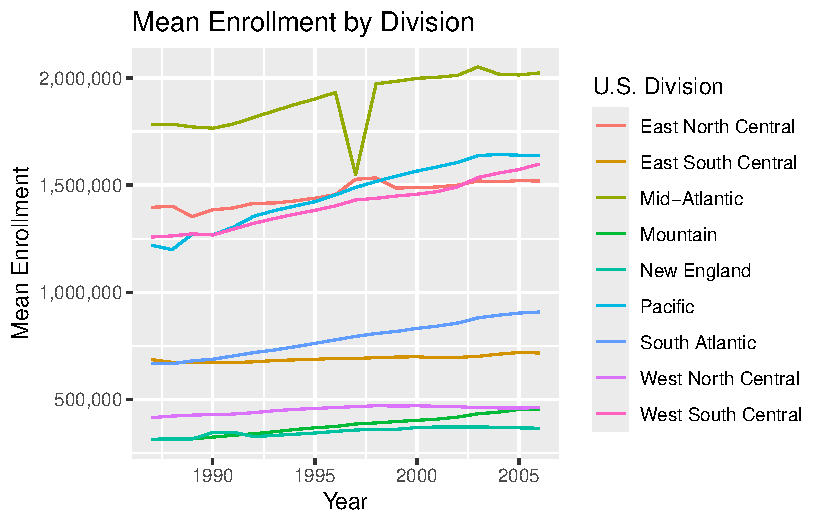
\includegraphics[keepaspectratio]{project1_files/figure-pdf/unnamed-chunk-30-1.pdf}}

Use the plot function on the county data frame

-- Once specifying the state to be ``NC'', the group being the top, the
number looked at being 20

\begin{Shaded}
\begin{Highlighting}[]
\FunctionTok{plot}\NormalTok{(one\_object[[}\DecValTok{1}\NormalTok{]], }\AttributeTok{top\_or\_bottom =} \StringTok{"top"}\NormalTok{, }\AttributeTok{n =} \DecValTok{20}\NormalTok{, }\AttributeTok{state =} \StringTok{"NC"}\NormalTok{)}
\end{Highlighting}
\end{Shaded}

\pandocbounded{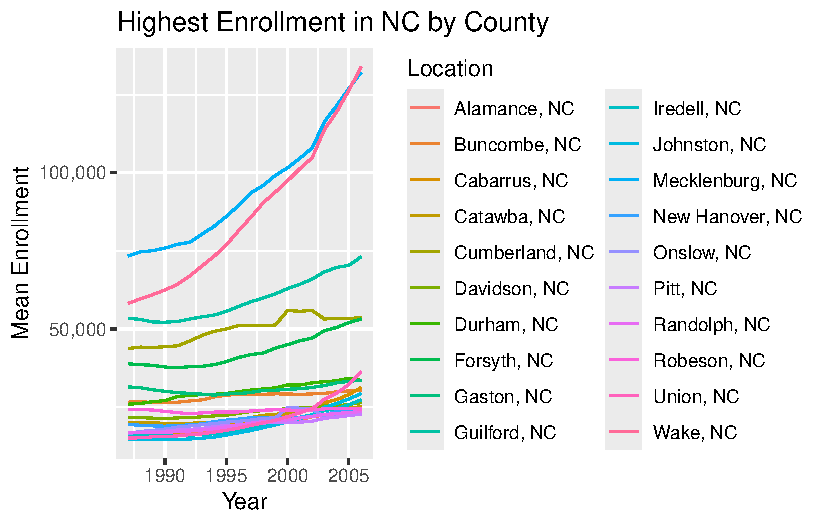
\includegraphics[keepaspectratio]{project1_files/figure-pdf/unnamed-chunk-31-1.pdf}}

-- Once specifying the state to be ``SC'', the group being the bottom,
the number looked at being 7

\begin{Shaded}
\begin{Highlighting}[]
\FunctionTok{plot}\NormalTok{(one\_object[[}\DecValTok{1}\NormalTok{]], }\AttributeTok{top\_or\_bottom =} \StringTok{"bottom"}\NormalTok{, }\AttributeTok{n =} \DecValTok{7}\NormalTok{, }\AttributeTok{state =} \StringTok{"SC"}\NormalTok{)}
\end{Highlighting}
\end{Shaded}

\pandocbounded{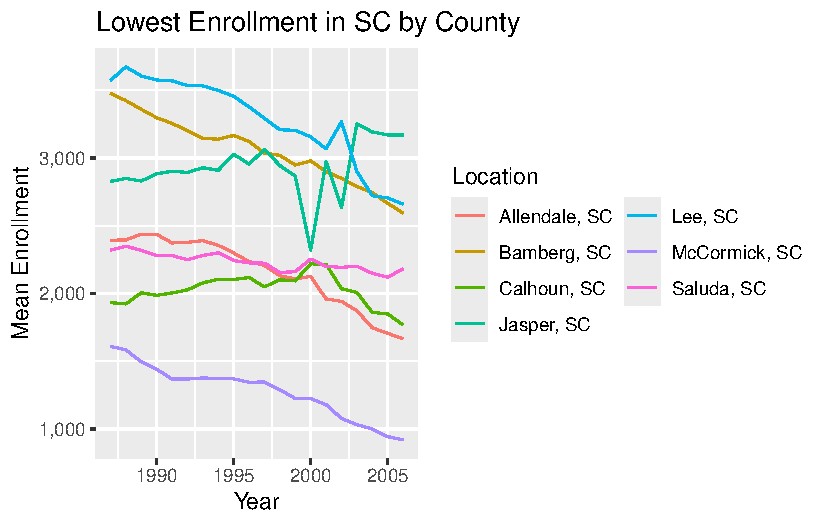
\includegraphics[keepaspectratio]{project1_files/figure-pdf/unnamed-chunk-32-1.pdf}}

-- Once without specifying anything (defaults used)

\begin{Shaded}
\begin{Highlighting}[]
\FunctionTok{plot}\NormalTok{(one\_object[[}\DecValTok{1}\NormalTok{]])}
\end{Highlighting}
\end{Shaded}

\pandocbounded{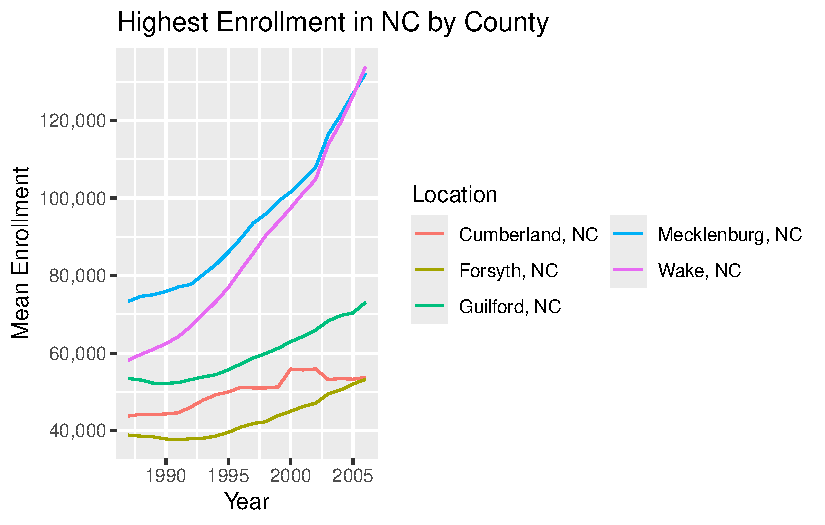
\includegraphics[keepaspectratio]{project1_files/figure-pdf/unnamed-chunk-33-1.pdf}}

-- Once specifying the state to be ``PA'', the group being the top, the
number looked at being 8

\begin{Shaded}
\begin{Highlighting}[]
\FunctionTok{plot}\NormalTok{(one\_object[[}\DecValTok{1}\NormalTok{]], }\AttributeTok{top\_or\_bottom =} \StringTok{"top"}\NormalTok{, }\AttributeTok{n =} \DecValTok{8}\NormalTok{, }\AttributeTok{state =} \StringTok{"PA"}\NormalTok{)}
\end{Highlighting}
\end{Shaded}

\pandocbounded{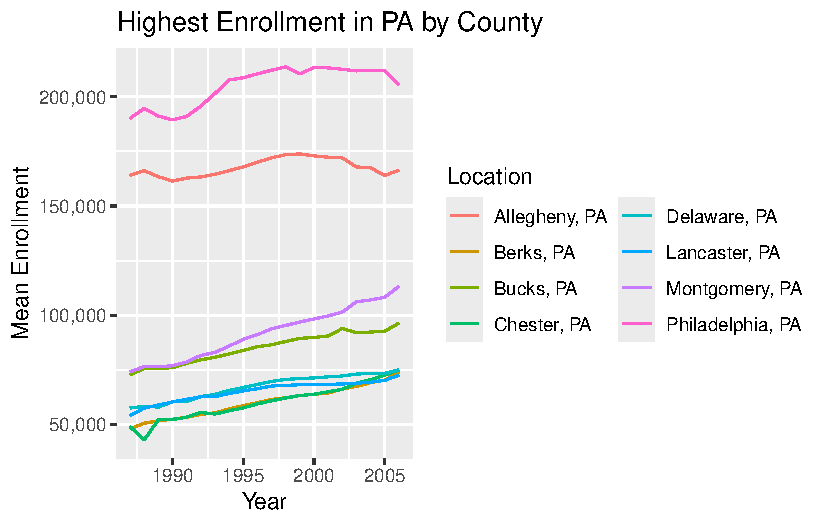
\includegraphics[keepaspectratio]{project1_files/figure-pdf/unnamed-chunk-34-1.pdf}}

Lastly, read in another couple similar data sets and apply your
functions!

Run your data processing function on the four data sets at URLs given.

\begin{Shaded}
\begin{Highlighting}[]
\NormalTok{dataPa }\OtherTok{\textless{}{-}} \FunctionTok{clean\_data\_wrapper}\NormalTok{(}\StringTok{"https://www4.stat.ncsu.edu/\textasciitilde{}online/datasets/PST01a.csv"}\NormalTok{)}
\end{Highlighting}
\end{Shaded}

\begin{verbatim}
[1] "Updating long data with year and measurement"
# A tibble: 5 x 4
  area_name     STCOU EDU_D      Enrollment
  <chr>         <chr> <chr>           <dbl>
1 UNITED STATES 00000 PST015171D  206827028
2 UNITED STATES 00000 PST015172D  209283904
3 UNITED STATES 00000 PST015173D  211357490
4 UNITED STATES 00000 PST015174D  213341552
5 UNITED STATES 00000 PST015175D  215465246
[1] "Assigning State to county tibble"
[1] "Assigning division to state tibble"
\end{verbatim}

\begin{Shaded}
\begin{Highlighting}[]
\NormalTok{dataPb }\OtherTok{\textless{}{-}} \FunctionTok{clean\_data\_wrapper}\NormalTok{(}\StringTok{"https://www4.stat.ncsu.edu/\textasciitilde{}online/datasets/PST01b.csv"}\NormalTok{)}
\end{Highlighting}
\end{Shaded}

\begin{verbatim}
[1] "Updating long data with year and measurement"
# A tibble: 5 x 4
  area_name     STCOU EDU_D      Enrollment
  <chr>         <chr> <chr>           <dbl>
1 UNITED STATES 00000 PST025182D  231665106
2 UNITED STATES 00000 PST025183D  233792697
3 UNITED STATES 00000 PST025184D  235825544
4 UNITED STATES 00000 PST025185D  237924311
5 UNITED STATES 00000 PST025186D  240133472
[1] "Assigning State to county tibble"
[1] "Assigning division to state tibble"
\end{verbatim}

\begin{Shaded}
\begin{Highlighting}[]
\NormalTok{dataPc }\OtherTok{\textless{}{-}} \FunctionTok{clean\_data\_wrapper}\NormalTok{(}\StringTok{"https://www4.stat.ncsu.edu/\textasciitilde{}online/datasets/PST01c.csv"}\NormalTok{)}
\end{Highlighting}
\end{Shaded}

\begin{verbatim}
[1] "Updating long data with year and measurement"
# A tibble: 5 x 4
  area_name     STCOU EDU_D      Enrollment
  <chr>         <chr> <chr>           <dbl>
1 UNITED STATES 00000 PST035191D  252980941
2 UNITED STATES 00000 PST035192D  256514224
3 UNITED STATES 00000 PST035193D  259918588
4 UNITED STATES 00000 PST035194D  263125821
5 UNITED STATES 00000 PST035195D  266278393
[1] "Assigning State to county tibble"
[1] "Assigning division to state tibble"
\end{verbatim}

\begin{Shaded}
\begin{Highlighting}[]
\NormalTok{dataPd }\OtherTok{\textless{}{-}} \FunctionTok{clean\_data\_wrapper}\NormalTok{(}\StringTok{"https://www4.stat.ncsu.edu/\textasciitilde{}online/datasets/PST01d.csv"}\NormalTok{)}
\end{Highlighting}
\end{Shaded}

\begin{verbatim}
[1] "Updating long data with year and measurement"
# A tibble: 5 x 4
  area_name     STCOU EDU_D      Enrollment
  <chr>         <chr> <chr>           <dbl>
1 UNITED STATES 00000 PST045200D  282171957
2 UNITED STATES 00000 PST045201D  285081556
3 UNITED STATES 00000 PST045202D  287803914
4 UNITED STATES 00000 PST045203D  290326418
5 UNITED STATES 00000 PST045204D  293045739
[1] "Assigning State to county tibble"
[1] "Assigning division to state tibble"
\end{verbatim}

Run your data combining function (probably three times) to put these
into one object (with two data frames)

\begin{Shaded}
\begin{Highlighting}[]
\NormalTok{once }\OtherTok{\textless{}{-}} \FunctionTok{combining\_tibbles}\NormalTok{(dataPa, dataPb)}

\NormalTok{twice }\OtherTok{\textless{}{-}} \FunctionTok{combining\_tibbles}\NormalTok{(once, dataPc)}

\NormalTok{thrice }\OtherTok{\textless{}{-}} \FunctionTok{combining\_tibbles}\NormalTok{(twice, dataPd)}
\end{Highlighting}
\end{Shaded}

Use the plot function on the state data frame

\begin{Shaded}
\begin{Highlighting}[]
\FunctionTok{plot}\NormalTok{(thrice[[}\DecValTok{2}\NormalTok{]])}
\end{Highlighting}
\end{Shaded}

\begin{verbatim}
`summarise()` has grouped output by 'division'. You can override using the
`.groups` argument.
\end{verbatim}

\pandocbounded{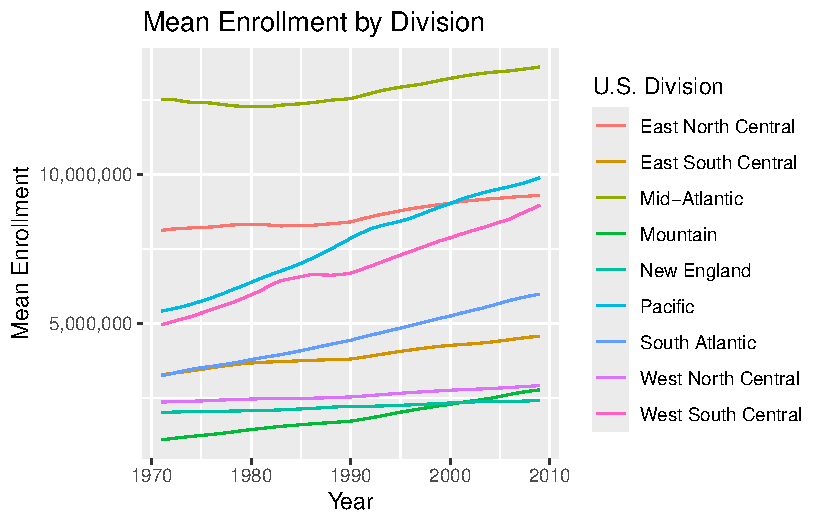
\includegraphics[keepaspectratio]{project1_files/figure-pdf/unnamed-chunk-37-1.pdf}}

Use the plot function on the county data frame -- Once specifying the
state to be ``CA'', the group being the top, the number looked at being
15

\begin{Shaded}
\begin{Highlighting}[]
\FunctionTok{plot}\NormalTok{(thrice[[}\DecValTok{1}\NormalTok{]], }\AttributeTok{top\_or\_bottom =} \StringTok{"top"}\NormalTok{, }\AttributeTok{n =} \DecValTok{15}\NormalTok{, }\AttributeTok{state =} \StringTok{"CA"}\NormalTok{)}
\end{Highlighting}
\end{Shaded}

\pandocbounded{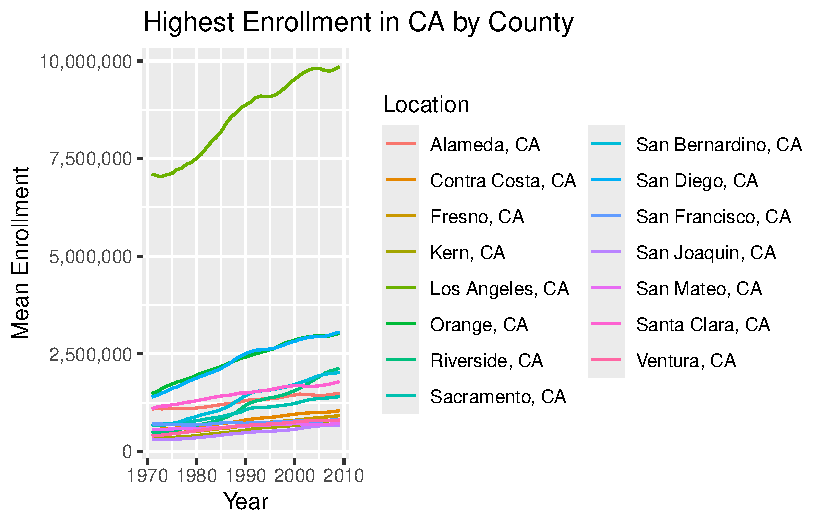
\includegraphics[keepaspectratio]{project1_files/figure-pdf/unnamed-chunk-38-1.pdf}}

-- Once specifying the state to be ``TX'', the group being the top, the
number looked at being 4

\begin{Shaded}
\begin{Highlighting}[]
\FunctionTok{plot}\NormalTok{(thrice[[}\DecValTok{1}\NormalTok{]], }\AttributeTok{top\_or\_bottom =} \StringTok{"top"}\NormalTok{, }\AttributeTok{n =} \DecValTok{4}\NormalTok{, }\AttributeTok{state =} \StringTok{"TX"}\NormalTok{)}
\end{Highlighting}
\end{Shaded}

\pandocbounded{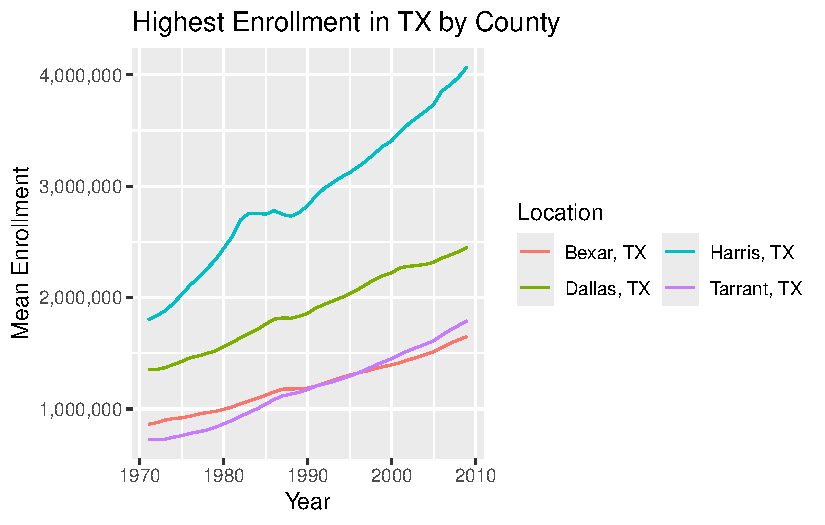
\includegraphics[keepaspectratio]{project1_files/figure-pdf/unnamed-chunk-39-1.pdf}}

-- Once without specifying anything (defaults used)

\begin{Shaded}
\begin{Highlighting}[]
\FunctionTok{plot}\NormalTok{(thrice[[}\DecValTok{1}\NormalTok{]])}
\end{Highlighting}
\end{Shaded}

\pandocbounded{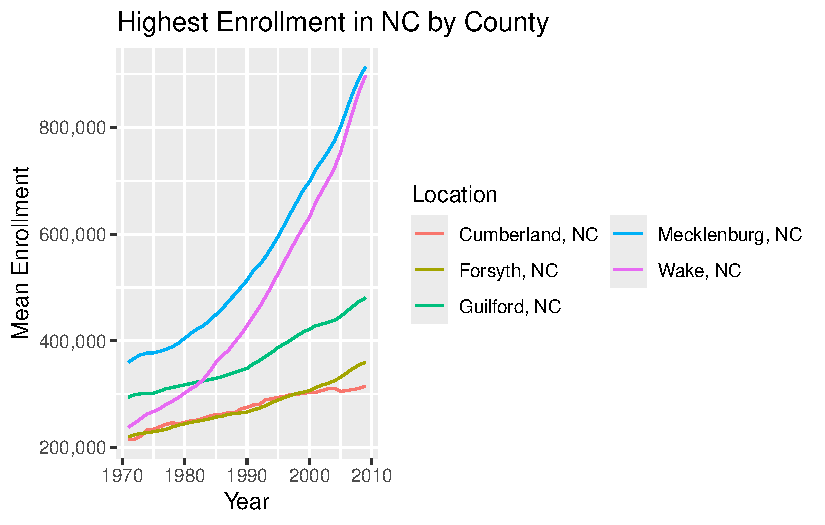
\includegraphics[keepaspectratio]{project1_files/figure-pdf/unnamed-chunk-40-1.pdf}}

-- Once specifying the state to be ``NY'', the group being the top, the
number looked at being 10

\begin{Shaded}
\begin{Highlighting}[]
\FunctionTok{plot}\NormalTok{(thrice[[}\DecValTok{1}\NormalTok{]], }\AttributeTok{top\_or\_bottom =} \StringTok{"top"}\NormalTok{, }\AttributeTok{n =} \DecValTok{10}\NormalTok{, }\AttributeTok{state =} \StringTok{"NY"}\NormalTok{)}
\end{Highlighting}
\end{Shaded}

\pandocbounded{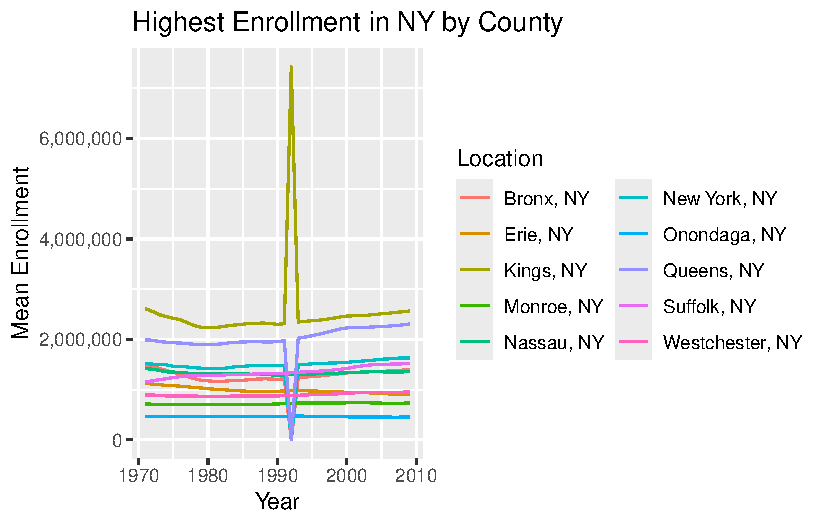
\includegraphics[keepaspectratio]{project1_files/figure-pdf/unnamed-chunk-41-1.pdf}}




\end{document}
